\documentclass[border=10pt]{standalone}
\usepackage[svgnames]{xcolor}
\usepackage{amsmath}
\usepackage{pgfplots}
\pgfplotsset{compat=newest}
\usepackage[sfdefault]{FiraSans}
\usepackage{FiraMono}
\renewcommand*\familydefault{\sfdefault}
\begin{document}
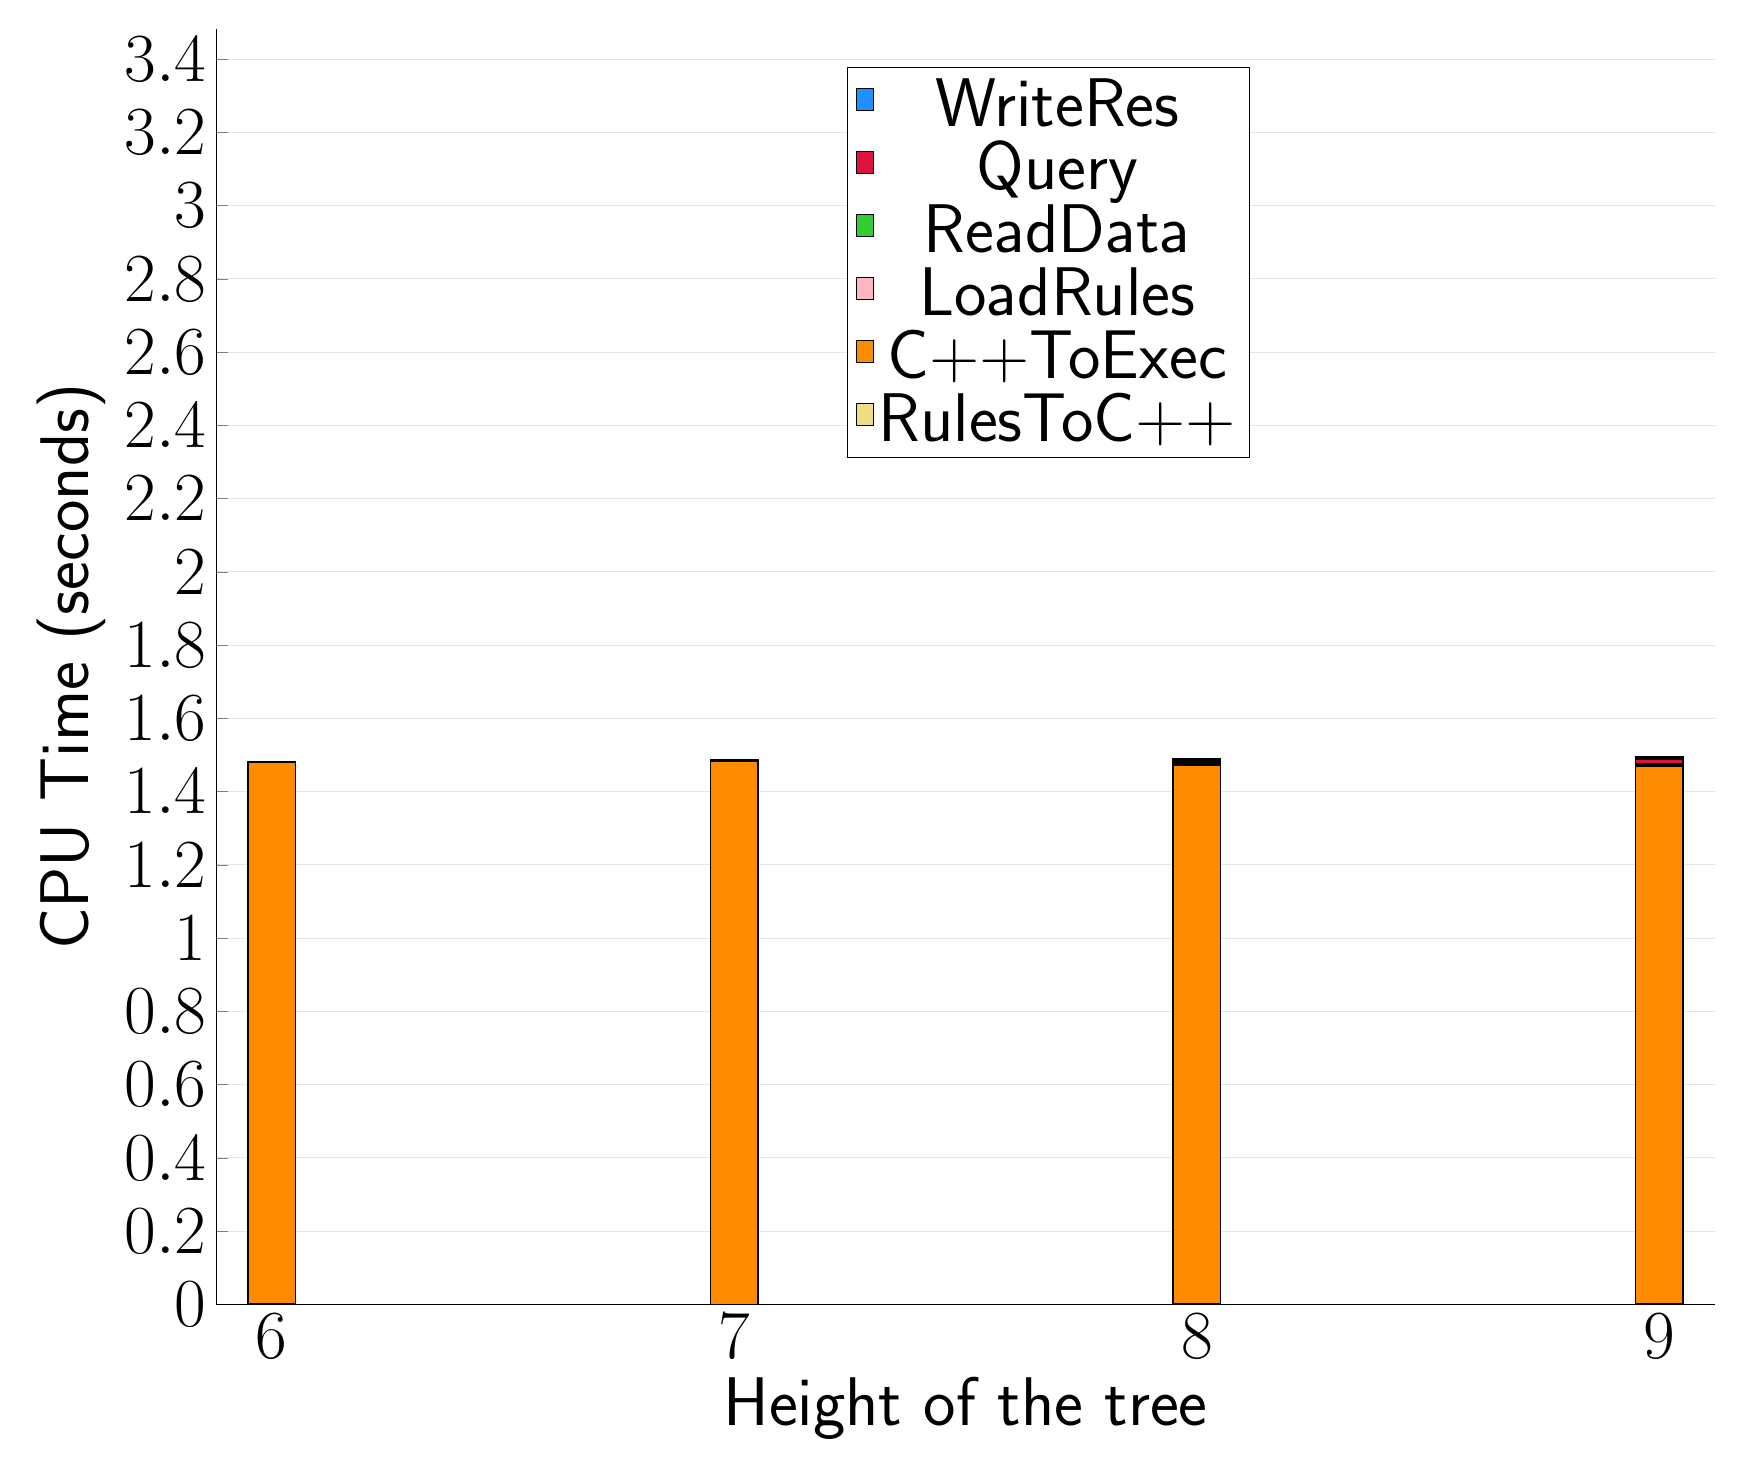
\begin{tikzpicture}
\begin{axis}[
   ybar stacked,
   width=1.7\textwidth,
   bar width=0.6cm,
   ymajorgrids, tick align=inside,
   major grid style={draw=gray!20},
   xtick=data,
   ymin=0, ymax=3.4819999999999998,
   axis x line*=bottom,
   axis y line*=left,
   enlarge x limits=0.04,
   legend style={
       at={(0.69, 0.97)},
       anchor=north east,
       legend columns=1,
       font=\Huge,
   },
   ylabel={CPU Time (seconds)},
   xlabel={Height of the tree},
   label style={font=\Huge},
   tick label style={font=\Huge},
]
\addlegendimage{fill=DodgerBlue, draw=black, line width=0.2pt}
\addlegendentry{WriteRes}
\addlegendimage{fill=Crimson, draw=black, line width=0.2pt}
\addlegendentry{Query}
\addlegendimage{fill=LimeGreen, draw=black, line width=0.2pt}
\addlegendentry{ReadData}
\addlegendimage{fill=LightPink, draw=black, line width=0.2pt}
\addlegendentry{LoadRules}
\addlegendimage{fill=DarkOrange, draw=black, line width=0.2pt}
\addlegendentry{C++ToExec}
\addlegendimage{fill=LightGoldenrod, draw=black, line width=0.2pt}
\addlegendentry{RulesToC++}
\addplot +[fill=LightGoldenrod, draw=black, line width=0.55pt] coordinates {
(6, 0.0020000000000000005)
(7, 0.0)
(8, 0.0020000000000000005)
(8, 0.0)
(8, 0.0)
(9, 0.0)
(9, 0.0020000000000000005)
(9, 0.0)
(9, 0.0)
(9, 0.0)
};
\addplot +[fill=DarkOrange, draw=black, line width=0.55pt] coordinates {
(6, 1.4780000000000002)
(7, 1.4819999999999998)
(8, 1.476)
(8, 1.476)
(8, 1.472)
(9, 1.474)
(9, 1.468)
(9, 1.468)
(9, 1.47)
(9, 1.468)
};
\addplot +[fill=LightPink, draw=black, line width=0.55pt] coordinates {
(6, 0.00017879999999999998)
(7, 0.0001746)
(8, 0.00019099999999999998)
(8, 0.0001766)
(8, 0.0001804)
(9, 0.000192)
(9, 0.0001842)
(9, 0.0001712)
(9, 0.0001856)
(9, 0.000177)
};
\addplot +[fill=LimeGreen, draw=black, line width=0.55pt] coordinates {
(6, 0.0006138000000000001)
(7, 0.0008704)
(8, 0.0013158)
(8, 0.0014463999999999998)
(8, 0.0014335999999999997)
(9, 0.0023284)
(9, 0.0023764)
(9, 0.0022728)
(9, 0.0023644)
(9, 0.002321)
};
\addplot +[fill=Crimson, draw=black, line width=0.55pt] coordinates {
(6, 0.0013384)
(7, 0.0033488)
(8, 0.008223600000000001)
(8, 0.0087268)
(8, 0.008762599999999999)
(9, 0.017195800000000004)
(9, 0.018335200000000003)
(9, 0.0176234)
(9, 0.017327600000000002)
(9, 0.017619199999999998)
};
\addplot +[fill=DodgerBlue, draw=black, line width=0.55pt] coordinates {
(6, 0.0005551999999999999)
(7, 0.0007661999999999999)
(8, 0.0009942)
(8, 0.0011896)
(8, 0.0011557999999999998)
(9, 0.0018886)
(9, 0.0017478)
(9, 0.0017582000000000001)
(9, 0.0017849999999999997)
(9, 0.0018435999999999997)
};
\end{axis}
\end{tikzpicture}

\end{document}
